\section{Source Code as Trees}\label{SourceCodeAsTrees}
As mentioned in the previous section the syntax analysis phase parses the source code into a tree.
Before this can be done the source code's symbols are separated into tokens adhering to the \acrshort{cfg} of \gls{gamble}.
These tokens are then further separated into the productions from the \acrshort{cfg}. 
These productions are recursive, and therefore a recursive data structure like a tree is compatible with the productions.
The tree structure is useful for this because every node of the tree can contain information and have references to its children as well as its parents. 
As a result it is possible to express the productions of a grammar by following a path on the tree from the root to a leaf.
A parse tree separates the source code into different productions of the grammar it represents, but also contains all of the syntax from the grammar, such as parentheses.
The tree structure makes it possible to traverse the tree in the same order as the source code is written, which means that the tree is not only able to express statements of the source code but also the order in which they are to be executed.\todo{Vi har jo godt nok forklaret hvad et parse træ var tidligere? What do. - Søren}
An example of a parse tree from the declaration \texttt{int a = 5;} is shown in \myref{image:PST}

\begin{figure}[ht]
    \centering
    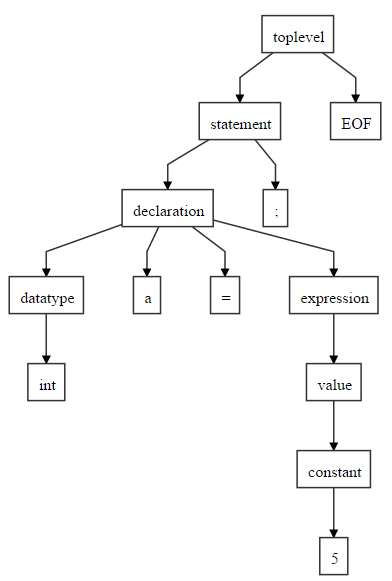
\includegraphics[width=0.5\linewidth]{figures/Trees/PST.PNG}
    \caption{A parse tree from the expression \texttt{int a = 5;} using \glspl{gamble} \acrshort{cfg}.}\label{image:PST}
\end{figure}

The next chapter will explain how the compiler creates a parser to produce the parse trees for the source code, and thus making it possible to use the trees in the compiler.
